%% Gene2Image -- IEEE TMI draft (expanded & polished; v2).
%% Compile: pdflatex main -> bibtex main -> pdflatex main -> pdflatex main
%% Requires IEEEtran.cls (standard; ships with TeX Live / MiKTeX).
%%
%% NOTE ON RESULTS: No full-scale (50-epoch, multi-seed) training has been run yet.
%% Every quantitative RESULT in this draft is a placeholder rendered as \TBD ([TBD]).
%% Populate them from results/summary_main.csv, results/ablation/summary.csv,
%% results/cross_dataset/summary.csv and results/interpret/<ds>/ after running
%% `bash code/scripts/run_all.sh <N>` on the GPU server. Protocol numbers
%% (datasets, gene counts, pathway counts, seeds, hyper-parameters, parameter
%% counts) are real and may stay. Forward-looking verbs ("is designed to",
%% "we expect", "is evaluated for") should be tightened to past-tense claims
%% ("improves", "reduces") only once the corresponding \TBD is filled.
%%
%% FIGURES: Fig.~1 (architecture schematic) is a complete TikZ figure. Figs.~2--3
%% (qualitative panels, attention maps) are self-compiling gray placeholders via
%% \figplaceholder; replace each with \includegraphics{figs/...} once the real
%% artwork exists.

\documentclass[journal]{IEEEtran}

\usepackage{amsmath,amssymb,amsfonts}
\usepackage{graphicx}
\usepackage{booktabs}
\usepackage{multirow}
\usepackage{array}
\usepackage[table]{xcolor}
\usepackage{tikz}
\usetikzlibrary{positioning, arrows.meta, fit, backgrounds}
\usepackage{algorithm}
\usepackage{algorithmic}
\usepackage{url}
\usepackage[hidelinks]{hyperref}

% Placeholder for unfilled experimental results.
\newcommand{\TBD}{{\color{red}\textbf{[TBD]}}}
\newcommand{\method}{Gene2Image}
\newcommand{\eg}{e.g.,}
\newcommand{\ie}{i.e.,}

% Self-compiling figure placeholder: #1 = height, #2 = descriptive caption text.
% Replace the whole \figplaceholder{...}{...} with \includegraphics once art exists.
\newcommand{\figplaceholder}[2]{%
  \setlength{\fboxsep}{6pt}%
  \fcolorbox{gray}{gray!8}{\parbox[c][#1][c]{0.96\linewidth}{%
    \centering\itshape\footnotesize\color{gray!55!black} #2}}}

\begin{document}

\title{Learnable Pathway Conditioning for Gene-Expression-to-Histopathology\\ Generation: A Controlled Study of Mechanism, Semantics, and Learnability}

\author{Anonymous Author(s)% <-- fill in author block before submission
\thanks{Manuscript draft. This work uses only publicly released Xenium data and
code; configurations and a single orchestration script that reproduces every
table are released with the project repository.}}

\markboth{IEEE Transactions on Medical Imaging (Draft)}%
{\method: Learnable Pathway Conditioning for Gene-to-Image Generation}

\maketitle

\begin{abstract}
Generating hematoxylin-and-eosin (H\&E) histopathology images from single-cell
gene expression is an emerging inverse problem. We
argue that the RNA conditioning encoder is a decisive, understudied bottleneck:
from high-dimensional ($\sim$300--5000 genes), sparse, noisy
expression it must distill a signal that is discriminative for morphology,
interpretable, and transferable across sequencing panels. Existing RNA conditioning approaches sit
at two extremes---an unstructured attention encoder that injects no biological
prior, and a fixed pathway-score conditioning representation (\eg\ ssGSEA-style)
that compresses expression before the generator, decoupling it from the
generative objective and potentially discarding within-pathway gene-level variation. \method\ adopts a learnable structured pathway bottleneck as the generator's
conditioning encoder, striking a middle ground between these extremes: a fixed pathway--gene binary mask welds
biological sparsity into the architecture, while a learnable weight vector on each
(pathway, gene) edge preserves gene-level resolution and lets the conditioning
adapt to the task. The encoder maps expression to pathway tokens, models pathway-token
dependencies with self-attention, and pools a CLS token whose attention
over pathways is a model-intrinsic interpretability signal. Reusing the
rectified-flow$+$UNet backbone unchanged, with its 512-dimensional conditioning
interface identical across variants, makes generation-quality differences
primarily attributable to the RNA conditioning encoder; under this controlled setup we decompose the pathway-prior benefit into
structured-sparsity and biological-semantics contributions, and compare a
learnable pathway bottleneck against a fixed pathway-score prior. On three Xenium
melanoma panels, \method\ is evaluated for generation fidelity, for cross-panel
transfer through a shared pathway space, and for pathway-to-morphology
explanations and their biological consistency and conditioning-sensitivity.
\end{abstract}

\begin{IEEEkeywords}
Computational pathology, spatial transcriptomics, conditional image generation,
rectified flow, biological pathways, interpretability, cross-panel transfer.
\end{IEEEkeywords}

\section{Introduction}
\IEEEPARstart{S}{patial} transcriptomics platforms such as 10x Xenium align
single-cell transcriptomes with the paired tissue morphology from which they were
measured, for the first time exposing, at cellular resolution, the map between
gene expression and histology~\cite{geneflow,hest}. This alignment has turned a
previously abstract question into a concrete learning problem: can we synthesize
an H\&E image directly from an expression profile? A positive answer would
enable virtual staining of unstained or degraded tissue, \emph{in-silico}
perturbation in which a hypothesized transcriptional change is rendered as a
predicted morphological change, augmentation of rare phenotypes for which paired
data are scarce, and---because the generator makes the gene$\rightarrow$morphology
dependence explicit---testable hypotheses about pathway-to-morphology associations~\cite{geneflow,rnacdm}. GeneFlow~\cite{geneflow}
is among the first methods to formulate this inverse mapping at single-cell resolution, coupling
an attention-based RNA encoder with a rectified-flow conditional UNet.

We take the position that the success of this inverse problem hinges on the RNA
\emph{conditioning encoder}, not on the generative backbone. From expression that
is high-dimensional, sparse, and noisy, the encoder must produce a conditioning
vector that is (i)~\emph{discriminative}, carrying the transcriptional signal that
actually predicts morphology; (ii)~\emph{interpretable}, so that a user can ask
\emph{which biological program drives a given morphological change} rather than
accept a black-box output; and (iii)~\emph{transferable}, so that a model trained
on one gene panel remains usable on another with a different gene set. Current
encoders satisfy none of the three cleanly, and in fact fall into two opposite
failure modes.

\textbf{Too little structure.} GeneFlow~\cite{geneflow} treats genes as
independent input features and, in the authors' own words, encodes ``no explicit
biological knowledge'' in its architecture. Confronted with thousands of
correlated, mostly uninformative dimensions, the encoder must discover biological
structure largely from the image-reconstruction signal alone, with no prior to
regularize the many correlated dimensions. The authors explicitly flag ``injecting
the biological structure of gene expression'' as the key direction for coping
with high-dimensional panels.

\textbf{Fixed, pre-compressed structure.} At the opposite extreme, the recent
multimodal foundation model MUPAD~\cite{mupad} introduces pathway information, but
as a \emph{fixed} pathway-score conditioning (ssGSEA-style)~\cite{ssgsea}: it reuses a predefined
pathway signature to compress genes into 331 pathway-level enrichment scores \emph{before} they
are injected into the generator. That compression is decoupled from the
generative objective and is not learnable; any gene-level variation the score
discards is permanently lost, and its interpretability is borrowed from an
external prior rather than learned by the model. The encoder is thus fixed and
pre-compressed exactly where it should adapt.

Pathways offer a natural middle ground. They organize tens of thousands of genes
into a few hundred functional modules, imposing sparse structure while preserving
within-module gene-level information. In discriminative settings, encoding
pathway priors into network structure improves both accuracy and interpretability
~\cite{pnet,survpath,tosica}. Yet in \emph{generation} tasks, how to inject
pathway structure into the conditioning signal has not been studied
systematically, and a more fundamental question remains open: \emph{does the
benefit of a pathway prior come from genuine biological semantics, or merely from
the structured sparsity it imposes?} ``Sparsity is All You Need''~\cite{sparsity}
found, across a range of discriminative models, that random pathway masks often match
real ones---attributing the gain to structured sparsity rather than biology---while
a P-NET reusability report~\cite{pnet_repro} quantified a real contribution
of Reactome sparsification in another discriminative setting, reaching a different
conclusion. Both bodies of
evidence are confined to discriminative tasks; the attribution in generation
has, to our knowledge, not been systematically evaluated.

We address these gaps with \method, which replaces GeneFlow's RNA encoder with an
end-to-end learnable structured pathway bottleneck and studies it under a
controlled protocol, leaving the generative backbone untouched
(Fig.~\ref{fig:overview}). A fixed pathway--gene
binary mask constrains which genes may influence which pathway (an expert-curated
structured biological prior), while a learnable weight vector on every retained (pathway, gene) edge
lets the model tune each gene's contribution to morphology (task adaptation)---the
two design axes that unstructured and fixed-scoring encoders each collapse. Because
the conditioning is emitted as a sequence of pathway tokens rather than a
gene-indexed vector, and because the pathway vocabulary is shared across panels,
the same encoder can transfer across gene sets, provided the shared pathways and
their member genes can be aligned. And because a CLS token aggregates the
pathway tokens through self-attention, the pathway-to-morphology map is an internal
product of the model that can be read out, compared to independent enrichment
analysis, and probed by intervening on individual pathway tokens.

Our contributions are:
\begin{itemize}
  \item \textbf{Structured pathway conditioning for generation.} We bring a
  mask-constrained learnable pathway encoder---a fixed pathway--gene binary mask
  with a learnable $D_{\text{token}}$-dimensional weight vector per non-zero
  (pathway, gene) pair---to gene-expression-to-image generation, filling the gap
  between GeneFlow's unstructured encoder and MUPAD's fixed pathway scoring. An
  edge-list scatter-add realizes the mapping without ever materializing the dense
  $P\times G\times D_{\text{token}}$ tensor, so the encoder is lightweight
  ($\sim$0.36\,M added parameters on Hallmark); the complete model's
  trainable-parameter count is reported against the unstructured baseline in
  Sec.~\ref{sec:impl}.
  \item \textbf{Model-intrinsic pathway interpretability.} Pathway-token
  self-attention with CLS aggregation makes the pathway-to-morphology importance a
  \emph{diagnostic} readout of the model's own attention rather than, as in
  MUPAD~\cite{mupad}, a precomputed external pathway score; the
  CLS$\rightarrow$pathway attention yields a per-cell pathway-importance profile
  that we evaluate for biological consistency and conditioning sensitivity---as an
  internal-consistency signal, not a causal explanation.
  \item \textbf{A controlled decomposition of the pathway-prior benefit in a
  generation task.} Through randPath (random same-density mask), PathPrior (frozen ssGSEA
  weights), noTrans, and noMask---each flipping a single orthogonal switch---we
  separate structured sparsity, biological semantics, pathway-token dependency
  modeling, and learnability under one generative-backbone architecture and
  conditioning interface, positioned
  to answer the question raised by~\cite{sparsity} and supplying the ``learnable
  vs.\ fixed'' ablation not reported by~\cite{mupad}.
  \item \textbf{A controlled, reproducible protocol.} By reusing the generative-backbone
  architecture unchanged---each variant trained end-to-end, the shared sampler
  carrying only variant-agnostic numerical corrections---and hard-aligning the
  512-dimensional conditioning interface, every reported difference is primarily
  attributable to the encoder; a single
  orchestration script reproduces all tables. All quantitative results in this
  draft are placeholders (\TBD) to be filled from that pipeline.
\end{itemize}

The remainder of the paper reviews related work (Sec.~\ref{sec:related}), details
the encoder, its variants, cross-panel transfer, and interpretability readout
(Sec.~\ref{sec:method}), specifies the experimental protocol
(Sec.~\ref{sec:experiments}), and discusses limitations
(Sec.~\ref{sec:discussion}).

\begin{figure*}[t]
\centering
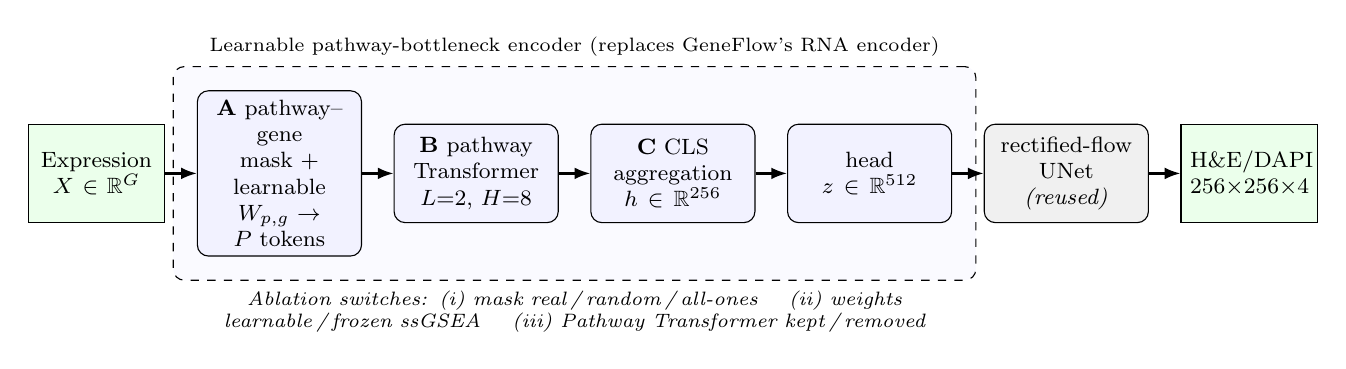
\begin{tikzpicture}[
  font=\footnotesize,
  node distance=4mm and 4mm,
  box/.style={draw, rounded corners, align=center, text width=1.85cm, minimum height=1.25cm, fill=blue!5},
  reused/.style={draw, rounded corners, align=center, text width=1.85cm, minimum height=1.25cm, fill=gray!12},
  io/.style={draw, align=center, text width=1.5cm, minimum height=1.25cm, fill=green!8},
  ar/.style={-{Latex[length=2mm]}, thick}
]
  \node[io] (x) {Expression\\ $X\in\mathbb{R}^{G}$};
  \node[box, right=of x] (a) {\textbf{A} pathway--gene\\ mask $+$ learnable\\ $W_{p,g}$ $\to$ $P$ tokens};
  \node[box, right=of a] (b) {\textbf{B} pathway\\ Transformer\\ $L{=}2,\,H{=}8$};
  \node[box, right=of b] (c) {\textbf{C} CLS\\ aggregation\\ $h\in\mathbb{R}^{256}$};
  \node[box, right=of c] (hd) {head\\ $z\in\mathbb{R}^{512}$};
  \node[reused, right=of hd] (u) {rectified-flow\\ UNet\\ \emph{(reused)}};
  \node[io, right=of u] (img) {H\&E/DAPI\\ $256{\times}256{\times}4$};
  \draw[ar] (x)--(a);
  \draw[ar] (a)--(b);
  \draw[ar] (b)--(c);
  \draw[ar] (c)--(hd);
  \draw[ar] (hd)--(u);
  \draw[ar] (u)--(img);
  \begin{scope}[on background layer]
    \node[draw, dashed, rounded corners, fill=blue!2, fit=(a)(b)(c)(hd), inner sep=3mm] (enc) {};
  \end{scope}
  \node[anchor=south, font=\scriptsize] at (enc.north)
    {Learnable pathway-bottleneck encoder (replaces GeneFlow's RNA encoder)};
  \node[anchor=north, align=center, font=\scriptsize\itshape, text width=9cm] at (enc.south)
    {Ablation switches: (i)~mask real\,/\,random\,/\,all-ones \quad
     (ii)~weights learnable\,/\,frozen ssGSEA \quad
     (iii)~Pathway Transformer kept\,/\,removed};
\end{tikzpicture}
\caption{Overview of \method. A fixed pathway--gene mask with learnable per-edge
weights maps per-cell expression to $P$ pathway tokens (A); a shallow pathway
Transformer models pathway-token interactions (B) and a CLS token aggregates them into a cell
embedding (C); a head emits the 512-d conditioning vector. The
rectified-flow$+$UNet backbone and its 512-d interface are reused unchanged
(identical architecture, retrained end-to-end per variant), so any quality change
is primarily attributable to the encoder. The three
orthogonal ablation switches shown below define all variants
(Table~\ref{tab:variants}).}
\label{fig:overview}
\end{figure*}

\section{Related Work}
\label{sec:related}

\subsection{Gene expression to histopathology generation}
Early work synthesized tissue tiles from \emph{bulk} RNA-seq. RNA-GAN~\cite{rnagan}
compresses expression with a variational autoencoder and generates tiles with a
GAN; RNA-CDM~\cite{rnacdm} instead uses a $\beta$-VAE encoder and a
cascaded-diffusion generator. Both operate at bulk resolution, model no spatial structure,
and discard inter-gene biology through generic dimensionality reduction.
GeneFlow~\cite{geneflow} is among the first to solve the map at single-cell resolution,
using a rectified-flow conditional UNet to produce high-resolution H\&E/DAPI
images and validating diagnostic plausibility by pathologist review; its RNA
encoder, however, injects no pathway prior. MUPAD~\cite{mupad} extends the
direction to a multimodal foundation model conditioned on \emph{fixed} ssGSEA
pathway scores. These works all connect transcriptomics to tissue images but differ
in input granularity and generative target---RNA-GAN and RNA-CDM at the bulk/tile
level, GeneFlow at single-cell resolution, and MUPAD as multimodal generation with
fixed pathway-level conditioning. From the RNA-conditioning perspective central to
this paper, they occupy two ends: GeneFlow uses an expression encoder without
explicit pathway structure, while MUPAD uses a precomputed fixed pathway-level
conditioning representation. How to inject pathway structure \emph{learnably} for
generation is, to our knowledge, understudied, and is the gap we target.

\subsection{Pathway-guided representation learning}
In discriminative settings, encoding pathway priors into network structure is
well established. P-NET~\cite{pnet} builds a hierarchical sparse network from
Reactome and recovers candidate drivers by node-importance analysis;
pmVAE~\cite{pmvae} constructs pathway-modular VAEs and explicitly handles the
gene overlap that makes pathways redundant; TOSICA~\cite{tosica} tokenizes genes
into pathway tokens, applies multi-head self-attention with a CLS token, and uses
the CLS attention as an interpretable cell embedding for annotation;
SurvPath~\cite{survpath} learns pathway tokens from transcriptomics and fuses them
with histology patches for survival prediction; PEaRL~\cite{pearl} encodes
transcriptomics as fixed, ssGSEA-style pathway-activation scores and aligns them with
histology by contrastive learning to predict gene- and pathway-level
expression---a discriminative histology$\to$expression setting, unlike our
RNA-conditioned generation. These methods all serve
classification or prediction objectives. \method\ follows the same broad design family as TOSICA~\cite{tosica}---a
pathway-token $+$ self-attention $+$ CLS encoder with a mask-constrained
\emph{learnable} embedding (a fixed biological mask with a learnable masked
projection, not a frozen transform)---and does not claim architectural novelty
over it. The difference is the
setting: TOSICA performs cell-type \emph{classification}, whereas \method\
repurposes this encoder as the conditioning pathway of a \emph{generative} model.
This shift is what enables our controlled decomposition of the pathway prior
(structured sparsity vs.\ pathway semantics; learnable vs.\ fixed ssGSEA),
cross-panel transfer through the shared pathway vocabulary, and a generative
pathway-intervention probe. We therefore do not claim the pathway-token
Transformer itself as a new architecture; our contribution lies in identifying
where the pathway prior's benefit comes from---and whether learnable pathway
conditioning improves over fixed pathway scores---when this encoder serves as the
conditioning interface for RNA-conditioned histology generation.

\subsection{Is the pathway prior necessary?}
The value of pathway priors has recently been contested. ``Sparsity is All You
Need''~\cite{sparsity} compared pathway-informed models against randomized
counterparts that preserve network sparsity but replace the biological wiring
with random connections, and found comparable---sometimes better---randomized
performance in its discriminative settings, suggesting that part of the gain may
stem from structured sparsity rather than pathway semantics. A P-NET reusability report~\cite{pnet_repro}
instead quantified a genuine contribution of Reactome sparsification in another
discriminative setting, reaching a different conclusion. This controversy is confined to discriminative tasks;
whether the benefit reflects structured sparsity or pathway semantics in
\emph{generation} remains, to our knowledge, untested.
\method\ treats ``random $\approx$ real'' as a hypothesis to test (through its
randPath variant), not an assumption to accept or reject a priori.

\subsection{Rectified-flow generation}
Rectified flow connects noise and data along near-straight, deterministic ODE
paths, improving training stability and few-step sampling. SD3~\cite{sd3} scales
it to high-resolution conditional synthesis, and GeneFlow~\cite{geneflow} applies
it to gene-to-image generation with a high-order ODE solver that copes with the
many-to-one nature of the map. We reuse this backbone's architecture
unchanged---each variant trained end-to-end, applying only variant-agnostic
numerical corrections to its sampler---so that the encoder is the only
architectural component changed across variants.

\subsection{Positioning}
Summarizing, existing conditioning encoders for gene-to-image generation sit
at two extremes: unstructured (GeneFlow~\cite{geneflow}, information overload, no
biological constraint) or fixed and pre-compressed (MUPAD~\cite{mupad}, information cut
off before the objective, not learnable). Whether the benefit of pathway structure
in generation reflects structured sparsity or genuine pathway semantics remains, to
our knowledge, untested, and
we are not aware of a controlled fixed-versus-learnable ablation of pathway
conditioning. \method\ sits between the two
extremes and turns each of these open questions into a controlled experiment.

\section{Method}
\label{sec:method}

\subsection{Overview}
\method\ reuses GeneFlow's rectified-flow conditional UNet unchanged and replaces only
the RNA encoder (Fig.~\ref{fig:overview}); the backbone is trained end-to-end for every
variant---its weights are not frozen, only its architecture and $512$-d conditioning
interface are held identical across variants. Our aim is not to reinvent the
pathway-token Transformer but to use it as the conditioning interface for
RNA-conditioned histology generation and, with this shared backbone, to test what
role pathway structure, semantics, and learnability play. For the single-cell entry point---our
main setting, chosen because it matches GeneFlow's primary results and exposes the
gene-importance analysis we use to validate interpretability---the encoder maps each
cell's expression to a sequence of pathway tokens through a fixed pathway--gene
mask with learnable per-edge weights (module A), models pathway-token interactions with
a shallow Transformer (module B), and pools a CLS token into a cell embedding
(module C). A final head projects the embedding to the 512-dimensional
conditioning vector expected by the UNet. For the multi-cell entry point,
GeneFlow's multi-head cell attention aggregates per-cell embeddings into the same
512-d vector. The data flow is
\begin{equation*}
\underbrace{X_{[B,G]}}_{\text{expression}} \!\rightarrow\!
\underbrace{T_{[B,P,D_t]}}_{\text{pathway tokens}} \!\rightarrow\!
\underbrace{h_{[B,D_c]}}_{\text{cell emb.}} \!\rightarrow\!
\underbrace{z_{[B,512]}}_{\text{condition}} \!\rightarrow\!
\underbrace{I_{[B,4,256^2]}}_{\text{H\&E/DAPI}} ,
\end{equation*}
where modules A--C are new and the final conditioning width is hard-aligned to
GeneFlow's $512$ so the UNet interface is unchanged. We use $D_{\text{token}}=48$,
a Transformer of $L{=}2$ layers and $H{=}8$ heads, and $D_c{=}256$.

\subsection{Pathway--gene mask embedding (module A)}
\label{sec:moduleA}
Let $X\in\mathbb{R}^{B\times G}$ be log1p-normalized expression and
$A\in\{0,1\}^{P\times G}$ a fixed binary mask with $A_{p,g}=1$ iff gene $g$
belongs to pathway $p$. For each non-zero pair $(p,g)$ we introduce a learnable
weight vector $W_{p,g}\in\mathbb{R}^{D_{\text{token}}}$ and a per-pathway bias
$b_p\in\mathbb{R}^{D_{\text{token}}}$. The token for pathway $p$ is
\begin{equation}
t_{p}[r] = \sum_{g:\,A_{p,g}=1} W_{p,g}[r]\cdot X_{g} + b_p[r], \quad r=1,\dots,D_{\text{token}}.
\label{eq:mask-embed}
\end{equation}
Equation~\eqref{eq:mask-embed} is a sparse linear transform constrained by $A$:
the mask fixes which genes can flow into which pathway (a structured biological prior),
while the learnable $W$ lets the model reweight each gene's contribution within
its pathway; combined with the $\ell_1$ penalty, this can encourage a sparser
gene-level usage pattern. This is
precisely the axis that unstructured and fixed-scoring encoders each collapse:
GeneFlow keeps the weights free but drops the mask, so there is no biological
constraint; MUPAD keeps a mask-like signature but freezes the weights (indeed
compresses them to a scalar), so the conditioning cannot adapt to the generative objective.

\textbf{Sparse realization and complexity.} Let $E=\lVert A\rVert_0$ be the number
of retained edges. Rather than instantiate the dense $P\times G\times
D_{\text{token}}$ weight tensor, we store an edge list $(\text{edge}_p,
\text{edge}_g)$ and compute~\eqref{eq:mask-embed} with a gather followed by a
\texttt{scatter\_add} (\ie\ \texttt{index\_add\_}) along the pathway axis
(Alg.~\ref{alg:encoder}). Peak activation memory is therefore
$O(N\!\cdot\!E\!\cdot\!D_{\text{token}})$ with $N=B$ (or $B\!\cdot\!C_{\max}$ in
the multi-cell case), never the dense $O(N\!\cdot\!P\!\cdot\!G\!\cdot\!
D_{\text{token}})$. Because Hallmark pathways are small ($E\ll P\cdot G$), the
embedding contributes only $\sim$0.36\,M parameters on the Hallmark protocol;
trainable-parameter counts against the unstructured GeneFlow encoder are reported
for transparency in Sec.~\ref{sec:impl}.

\textbf{Mask construction.} We build $A$ per dataset from MSigDB Hallmark gene
sets~\cite{hallmark} intersected with that panel's genes by exact symbol matching
(no alias resolution; pathway genes absent from the panel are ignored), dropping
pathways with fewer than three retained genes; the column order of $A$ is aligned gene-by-gene to the dataset's
\texttt{gene\_names} to prevent silent index misalignment. An $\ell_1$ penalty
$\lambda\lVert W\rVert_1$ (with $\lambda=10^{-3}$) encourages the implicit feature
selection above and inherits the role of GeneFlow's first-layer $\ell_1$ term.

\begin{algorithm}[t]
\caption{Pathway-bottleneck encoder (single-cell forward)}
\label{alg:encoder}
\begin{algorithmic}[1]
\STATE \textbf{Input:} expression $X\in\mathbb{R}^{N\times G}$; edge lists
$\text{edge}_p,\text{edge}_g\in\mathbb{Z}^{E}$; weights $W\in\mathbb{R}^{E\times
D_t}$; bias $b\in\mathbb{R}^{P\times D_t}$
\STATE $X_{\text{edge}} \leftarrow X[:,\text{edge}_g]$ \hfill $\triangleright\ [N,E]$
\STATE $C \leftarrow X_{\text{edge}}[:,:,\text{None}] \odot W[\text{None},:,:]$ \hfill $\triangleright\ [N,E,D_t]$
\STATE $T \leftarrow \mathbf{0}^{N\times P\times D_t}$;\ \ $T.\texttt{index\_add\_}(1,\ \text{edge}_p,\ C)$
\STATE $T \leftarrow T + b[\text{None},:,:]$ \hfill $\triangleright$ pathway tokens $[N,P,D_t]$
\STATE $S \leftarrow [\,\texttt{CLS};\, T\,]$ \hfill $\triangleright\ [N,P{+}1,D_t]$
\STATE $S' \leftarrow \textsc{TransformerEncoder}_{L,H}(S)$ \COMMENT{no positional enc.}
\STATE $h \leftarrow \textsc{Proj}(S'[:,0])$ \hfill $\triangleright$ cell emb. $[N,D_c]$
\STATE $z \leftarrow \textsc{Head}(h)$ \hfill $\triangleright$ condition $[N,512]$
\STATE \textbf{return} $z$;\ \ export $\alpha_{\text{cls}\to p}$ from the last layer's head-averaged attention
\end{algorithmic}
\end{algorithm}

\subsection{Pathway Transformer and CLS aggregation (modules B, C)}
The $P$ pathway tokens of a cell are processed by an $L{=}2$-layer, $H{=}8$-head
Transformer encoder (feed-forward width $4D_{\text{token}}$, pre-norm). We omit
positional encoding because pathways are an unordered set; self-attention models
statistical dependencies among pathway tokens---which may reflect co-regulation
via shared proteins or cross-talk (\eg\ between cell-cycle and DNA-repair
programs), though we do not read attention as direct biological regulation. A learnable CLS token is prepended, and
its output is projected to the cell embedding $h\in\mathbb{R}^{D_c}$, $D_c{=}256$.
The CLS$\rightarrow$pathway attention $\alpha_{\text{cls}\to p}$, taken from the
last Transformer layer and averaged over heads, is exported as a model-internal
diagnostic of conditioning use---not a direct measure of causal pathway importance---for the analyses of Sec.~\ref{sec:interp}. A
final head $\mathrm{LN}\!\rightarrow\!\mathrm{Linear}\!\rightarrow\!\mathrm{LN}$
maps $h$ to the $512$-d conditioning vector. For the multi-cell entry point,
per-cell embeddings are aggregated by GeneFlow's multi-head cell attention
(padding masked by valid-cell counts) into the same $512$-d vector, so the two
entry points share every component except cell aggregation.

\subsection{Generative backbone (reused unchanged, trained per variant)}
The conditioning vector is injected into GeneFlow's rectified-flow conditional
UNet exactly as in the original: an MLP projects $z$ and adds it to the timestep
embedding, which modulates residual blocks by scale-shift normalization. Training
regresses the velocity field of GeneFlow's sinusoidal noise-to-data schedule
$x(t)=\sin(\tfrac{\pi}{2}t)\,x_1+(1-\sin(\tfrac{\pi}{2}t))\,x_0$ (with $x_0$
Gaussian noise; a small time-decaying stochastic term is additionally added to
$x(t)$ during training),
\begin{equation}
\mathcal{L}_{\text{flow}}=\mathbb{E}_{x_0,x_1,t}\big\lVert v_\theta(x(t),t,z)-\tfrac{\pi}{2}\cos(\tfrac{\pi}{2}t)\,(x_1-x_0)\big\rVert^2,
\label{eq:flow}
\end{equation}
and inference integrates the learned ODE from noise to image with a high-order
solver~\cite{geneflow,sd3}. The full training objective is
$\mathcal{L}=\mathcal{L}_{\text{flow}}+\lambda\lVert W\rVert_1$. We reuse the UNet
and the rectified-flow velocity parameterization unchanged---the backbone is trained
end-to-end for every variant, not frozen; the only backbone-side
edits are two numerical corrections to the shared Dormand--Prince sampler
(integrating fully to $t{=}1$ and correcting the adaptive step-size error
estimate), which alter no trained weights and apply identically to every variant.
With the $512$-d interface identical across variants, any quality difference is primarily
attributable to the RNA conditioning encoder.

\subsection{Controlled variants}
\label{sec:variants}
All variants are combinations of three orthogonal binary switches: the
\emph{mask} (real Hallmark / random same-density / all-ones), the
\emph{(pathway, gene) weights} (learnable / frozen ssGSEA), and the
\emph{Pathway Transformer} (kept / removed). Each ablation flips exactly one
switch relative to the full method, so differences are primarily attributable to
the encoder switch (Table~\ref{tab:variants}).

\begin{table}[t]
\centering
\caption{Model variants as three orthogonal switches. Each ablation flips one switch relative to \method.}
\label{tab:variants}
\renewcommand{\arraystretch}{1.2}
\begin{tabular}{@{}lcccl@{}}
\toprule
Variant & Mask & Weights & Transf. & Tests \\
\midrule
\textbf{\method} & real & learnable & \checkmark & RQ1 (full) \\
GeneFlow~\cite{geneflow} & --- & --- & --- & baseline / lower bound \\
randPath & random & learnable & \checkmark & RQ2 semantics \\
PathPrior & real & frozen ssGSEA & \checkmark & RQ3: learnable vs.\ fixed \\
noTrans & real & learnable & $\times$ & pathway-token interactions \\
noMask & all-ones & learnable & \checkmark & structured sparsity \\
\bottomrule
\end{tabular}
\end{table}

\textbf{PathPrior (RQ3).} To isolate ``learnable vs.\ fixed,'' PathPrior freezes
the per-edge weights $W$ (\texttt{requires\_grad=False}) at fixed values and the
per-pathway bias $b$ at its zero initialization, while keeping tokenization and
the Pathway Transformer intact---so the only switch flipped relative to \method\
is learnability of the within-pathway gene weighting (a single-scalar-per-pathway
version would additionally remove tokenization and entangle the comparison with
noTrans). Each fixed weight is derived from full-panel statistics: within a
retained pathway, gene $g$ is weighted by its mean expression over all cells
(including the held-out evaluation cells; see Sec.~\ref{sec:discussion}), and the
weights are normalized to sum to one over the pathway's genes (with a uniform
$1/k_p$ fallback when a pathway's members all have zero mean expression). The
resulting per-edge scalar then scales a fixed, seed-fixed, zero-mean unit-norm
$D_{\text{token}}$ profile rather than being broadcast identically across
$D_{\text{token}}$: a constant token would be centred out by the pre-norm
LayerNorm and make the conditioning input-independent; the profile is shared
across variants and seeds. This
expression-derived, ssGSEA-style weighting is a more faithful proxy for enrichment
scoring than uniform $1/k_p$. PathPrior is thus an in-framework proxy for
MUPAD-style fixed pathway-score conditioning, not a reproduction of the full MUPAD
system---which would additionally differ in backbone, bulk pretraining, and scalar
compression, and whose weights are not public.

\textbf{randPath (RQ2).} The random mask preserves each pathway's gene count but
shuffles gene membership, reproducing the ``randomized-but-structure-preserving''
setup of~\cite{sparsity}. \method\ vs.\ randPath then measures the added value of
real biological \emph{semantics} at matched parameter count and architecture---the
cleanest control in the study---while structured sparsity itself is isolated by
\method\ vs.\ noMask. The randPath vs.\ GeneFlow gap reflects the \emph{total}
benefit of the pathway-token encoder over the unstructured baseline, since the two
also differ in tokenization and the Transformer, not sparsity alone.

\textbf{noTrans, noMask.} noTrans removes the Pathway Transformer (CLS reduces to
a mean over pathway tokens), isolating the value of modeling pathway-token
interactions. noMask replaces the sparse mask with an all-ones matrix so every
token sees every gene, probing the value of structured sparsity; because noMask
has substantially more parameters, its failing to beat \method\ would support
sparsity, whereas its winning could not be attributed to removing the mask alone.

\subsection{Cross-panel transfer}
Because the conditioning is a $P$-token pathway sequence rather than a
$G$-dimensional gene vector, a model trained on one panel can be evaluated on
another whose genes differ, provided the two panels share pathway \emph{names}.
Hallmark defines a common vocabulary of up to $50$ pathways; after the
$\geq 3$-gene filter each panel retains a subset (Table~\ref{tab:datasets}), and
transfer uses the \emph{intersection of the retained pathway names}, each panel
keeping its own gene columns. We align the source and target masks to this shared,
identically ordered pathway list; at target evaluation the encoder is rebuilt on
the target mask; each target (pathway, gene) edge whose pathway \emph{and} gene
names both appear in the source receives the source-trained weight, while
target-only edges (genes or pathways absent from the source) keep their default
initialization. Per-pathway biases transfer by pathway name, and the Pathway
Transformer, CLS head, conditioning head, and UNet load unchanged. GeneFlow has
no such intermediate layer: its gene-indexed encoder's input dimension equals the
gene count, so it cannot transfer across mismatched panels without ad-hoc padding
or truncation, and is reported as not applicable; we read this N/A as
incompatibility of its input interface with the transfer protocol, not as lower
performance.

\subsection{Interpretability readout}
\label{sec:interp}
For a trained \method, the per-cell CLS$\rightarrow$pathway attention yields a
pathway-importance profile. We probe it along three increasingly demanding axes.
\emph{(A) Endogeneity.} We report attention entropy $-\sum_p \alpha_p\log\alpha_p$
(low entropy $\Rightarrow$ focused rather than uniform use of the pathway
structure) and, per cell type, the dominant pathways and their cross-type Jaccard
distinctiveness. \emph{(B) Biological consistency.} We compute the top-$k$ overlap
and Spearman correlation between the model's dominant pathways and pathways
enriched from GeneFlow's gene-importance scores on the same data (gene set
enrichment analysis, GSEA~\cite{gsea}, with a gene-rank-percentile enrichment
fallback when \texttt{gseapy} is unavailable). Because the training objective never supervises pathway
importance, such agreement---if it appears---would indicate that the model's
internal pathway use aligns with an independent gene-importance analysis, which
randPath (lacking biological semantics) should not reproduce. \emph{(C) Conditioning sensitivity.} We intervene on a
single pathway token at inference (ablate it to zero, or amplify it) while sharing
the initial generative noise across the base and intervened runs (so the shift
reflects the intervention, not sampling variance), and measure the resulting
morphological shift; the ratio of shift for dominant versus random pathways is a
specificity score.

\section{Experiments}
\label{sec:experiments}
\emph{All quantitative results below are placeholders (\TBD) pending the full
multi-seed training run; the protocol, datasets, pathway counts, and
hyper-parameters are final.}

\subsection{Datasets and protocol}
We use the three preprocessed Xenium human-skin melanoma samples released by
GeneFlow~\cite{geneflow} (Zenodo \texttt{records/17429142}); see
Table~\ref{tab:datasets}. Expression is log1p-normalized; images are
$256\times256\times4$ (H\&E RGB $+$ DAPI). Following GeneFlow's released code, each
panel uses a single random $80/20$ split with the evaluation set also used as
validation; this limits the interpretation of \emph{absolute} metrics
(Sec.~\ref{sec:discussion}), but all variants share the same split, hyper-parameters,
and training budget, so the protocol is most appropriate for \emph{relative}
comparisons. Given the cost of full generative training, we use three seeds
$\{42,43,44\}$ to estimate run-to-run variability---reporting per-seed values and
their mean$\pm$std and emphasizing effect sizes relative to seed variance rather
than significance testing---and fix the sampling noise so that seeds control the
data split and initialization (and, for randPath, the per-seed random-mask draw;
see Sec.~\ref{sec:discussion}). Pathway masks are built per
panel from MSigDB Hallmark (up to $50$ pathways, $33/40/50$ retained on C1/C2/P1
after filtering), with an optional Hallmark$+$Reactome~\cite{reactome} extension on the largest
panel ($P{=}1666$); Reactome is included only as a reference-scale pathway
vocabulary and is not independently evaluated in the reported protocol.

\begin{table}[t]
\centering
\caption{Datasets (GeneFlow Xenium melanoma panels). $P$ = Hallmark pathways retained after the $\geq 3$-gene filter.}
\label{tab:datasets}
\renewcommand{\arraystretch}{1.2}
\begin{tabular}{@{}llrrr@{}}
\toprule
ID & Panel & Genes $G$ & Pathways $P$ & Patches / Cells \\
\midrule
C1 & Base FFPE       & 282  & 33 & 9{,}394 / 106{,}980 \\
C2 & Add-on FFPE     & 382  & 40 & 39{,}334 / 70{,}178 \\
P1 & Prime FFPE      & 5006 & 50 & 13{,}832 / 137{,}927 \\
\bottomrule
\end{tabular}
\end{table}

\textbf{Implementation.}
\label{sec:impl}
We use the single-cell model, image size $256$, $4$ channels; AdamW
(lr $10^{-4}$, weight decay $10^{-2}$), cosine schedule, $50$ epochs, batch size
$16$, gradient clipping $1.0$, mixed precision, and $\ell_1$ weight $10^{-3}$;
generation uses a high-order ODE solver with up to $100$ steps. The reported
checkpoint is the epoch of lowest validation velocity-MSE---the flow-matching
term of Eq.~\ref{eq:flow} alone, excluding the $\ell_1$ penalty---selected with
early stopping (patience $5$). We select on this $\ell_1$-free velocity-MSE rather
than the total validation loss because the $\ell_1$ magnitude differs by orders of
magnitude across the encoder variants (free RNA weights vs.\ sparse pathway edge
weights vs.\ the all-ones mask), so selecting on the full loss would snapshot each
variant at a different point on its learning curve; the velocity-MSE is identically
defined across all variants, keeping the ablation fair. This is a deliberate,
variant-agnostic deviation from GeneFlow's total-loss checkpoint selection. The
encoder uses $D_{\text{token}}{=}48$, $L{=}2$, $H{=}8$, $D_c{=}256$. The pathway embedding adds
$\sim$0.36\,M parameters (Hallmark). All variants reuse the same
rectified-flow$+$UNet backbone architecture and the same $512$-d conditioning
interface, so differences are not confounded by changes in the generative-backbone
architecture or the conditioning-interface dimension. Trainable-parameter counts
under the single-cell configuration (RNA encoder $+$ UNet), reported only for
transparency, are \method\ $\approx$\TBD\,M versus GeneFlow $\approx$\TBD\,M
(to be counted uniformly on the released configuration). All variants share these settings;
only the switches of Table~\ref{tab:variants} differ.

\textbf{Metrics.} Following GeneFlow~\cite{geneflow}: FID (Inception features,
reported as an overall FID over the evaluation set; per-batch FID is computed but
not used for ranking, as it is sensitive to batch size), SSIM and PSNR (on the
three RGB channels, per-sample, excluding the DAPI channel), and a
pathology-foundation-model FID computed in UNI2-h features~\cite{uni,uni2h}; cross-panel
transfer additionally reports the degradation rate
$(\mathrm{FID}_{\text{cross}}-\mathrm{FID}_{\text{same}})/\mathrm{FID}_{\text{same}}$.
We treat FID/SSIM/PSNR as public, backbone-independent metrics (using only
publicly available feature extractors) and UNI2-h FID as an optional
pathology-specific metric reported when its gated checkpoint is available, so the
core comparison never depends on gated weights. Interpretability reports attention
entropy, top-$k$ overlap and Spearman correlation with GSEA, and the intervention
specificity ratio.

\subsection{Main results (RQ1)}
Table~\ref{tab:main} compares \method\ with the unstructured GeneFlow baseline
under the identical backbone and protocol. We use P1, the highest-dimensional panel, as the most stringent test of whether
structured sparsity helps under high-dimensional gene panels; on the
low-dimensional C1/C2 panels, which carry less uninformative signal to suppress,
any difference is expected to be smaller. Fig.~\ref{fig:qual} will present
qualitative comparisons alongside the reference H\&E once training completes.

\begin{table}[t]
\centering
\caption{Main comparison: generation quality (mean$\pm$std over 3 seeds). $\downarrow$/$\uparrow$: lower/higher is better. Numbers pending full training.}
\label{tab:main}
\renewcommand{\arraystretch}{1.2}
\begin{tabular}{@{}lcccc@{}}
\toprule
Method & FID$\downarrow$ & SSIM$\uparrow$ & PSNR$\uparrow$ & UNI2-h FID$\downarrow$ \\
\midrule
GeneFlow~\cite{geneflow} & \TBD & \TBD & \TBD & \TBD \\
\textbf{\method} & \TBD & \TBD & \TBD & \TBD \\
\bottomrule
\end{tabular}
\end{table}

\begin{figure}[t]
\centering
\figplaceholder{4.2cm}{Fig.~2 (to be added): qualitative generation on C1/C2/P1.
Rows: reference H\&E/DAPI, GeneFlow, \method. Columns: representative cells across
cell types. Insets highlight nuclear morphology where structured conditioning is
expected to sharpen boundaries. Populate from \texttt{results/<variant>\_<ds>\_seed42/}.}
\caption{Qualitative comparison of generated histopathology (placeholder).}
\label{fig:qual}
\end{figure}

\subsection{Ablation: structured sparsity vs.\ semantics, and learnable vs.\ fixed (RQ2, RQ3)}
Table~\ref{tab:ablation} flips one switch at a time. \method\ vs.\ randPath
isolates real pathway semantics at matched parameters and architecture (RQ2);
\method\ vs.\ noMask isolates structured sparsity (sparse vs.\ dense connectivity,
noMask carrying more parameters); \method\ vs.\ PathPrior isolates learnability
(RQ3); \method\ vs.\ noTrans isolates pathway-token interactions. The randPath vs.\
GeneFlow gap should be read as the \emph{total} benefit of the pathway-token
encoder over the unstructured baseline, not of sparsity alone. These variants jointly test whether the benefit arises from biological pathway
semantics (\method\ vs.\ randPath), structured sparsity (\method\ vs.\ noMask),
pathway-token learnability (\method\ vs.\ PathPrior), or pathway-token interactions
(\method\ vs.\ noTrans). Should randPath match \method, we read the benefit as
coming mainly from structured sparsity (learnably injected) rather than pathway
semantics, which \emph{weakens} the biological-semantics claim rather than
confirming it.

\begin{table}[t]
\centering
\caption{Ablation on C1 and P1 (FID$\downarrow$ / UNI2-h FID$\downarrow$). Each variant flips one switch vs.\ \method. Numbers pending full training.}
\label{tab:ablation}
\renewcommand{\arraystretch}{1.2}
\begin{tabular}{@{}lccl@{}}
\toprule
Variant & C1 & P1 & Flipped switch \\
\midrule
GeneFlow & \TBD & \TBD & no pathway encoder \\
randPath & \TBD & \TBD & real $\to$ random mask \\
PathPrior & \TBD & \TBD & learnable $\to$ frozen \\
noTrans & \TBD & \TBD & remove Transformer \\
noMask & \TBD & \TBD & sparse $\to$ dense \\
\textbf{\method} & \TBD & \TBD & full \\
\bottomrule
\end{tabular}
\end{table}

\subsection{Cross-panel transfer}
Table~\ref{tab:cross} trains on a source panel and evaluates on a target panel
through the shared pathway space (C1$\to$C2, C2$\to$C1, C1$\to$P1). Because
GeneFlow's gene-indexed encoder has an input dimension equal to the gene count, it
cannot be applied to a mismatched panel without ad-hoc padding or truncation; its
N/A entries denote this structural inapplicability, not measured degradation. We
therefore report \method's own same-panel-versus-cross-panel degradation rate
(not compared against GeneFlow), expected to be largest on the hardest
small-to-large C1$\to$P1 setting. All transfer settings are within melanoma Xenium
panels; we do not claim cross-tissue or cross-organ generalization.

\begin{table}[t]
\centering
\caption{Cross-panel transfer. Degradation rate $=(\mathrm{FID}_{\text{cross}}-\mathrm{FID}_{\text{same}})/\mathrm{FID}_{\text{same}}$ (lower better). Numbers pending full training.}
\label{tab:cross}
\renewcommand{\arraystretch}{1.2}
\begin{tabular}{@{}llcc@{}}
\toprule
Model & Setting & FID$_{\text{cross}}\downarrow$ & Degradation$\downarrow$ \\
\midrule
GeneFlow~\cite{geneflow} & C1$\to$P1 & N/A & N/A \\
\textbf{\method} & C1$\to$C2 & \TBD & \TBD \\
\textbf{\method} & C2$\to$C1 & \TBD & \TBD \\
\textbf{\method} & C1$\to$P1 & \TBD & \TBD \\
\bottomrule
\end{tabular}
\end{table}

\subsection{Pathway interpretability (RQ4)}
We test whether the pathway attention is (A) endogenous, (B) biologically
consistent, and (C) conditioning-sensitive (Sec.~\ref{sec:interp}); Fig.~\ref{fig:interp} will
visualize per-cell-type attention and an intervention example. \emph{(A)} We report per-cell-type attention entropy against the uniform bound
$\log P$ (\TBD); lower entropy indicates focused rather than uniform pathway use. \emph{(B)} The model's dominant pathways are compared with GeneFlow
gene-importance GSEA pathways by top-$k$ overlap (\TBD) and Spearman correlation
(\TBD); if biological pathway semantics matter, randPath should show weaker
agreement under the same evaluation. Because both models train on the same data,
this cross-model agreement is a necessary but not sufficient check. \emph{(C)} We measure whether intervening on
dominant pathways produces larger morphological shifts than intervening on random
pathways (specificity ratio \TBD), a model-internal conditioning-sensitivity
probe---not a biological causal claim.

\begin{figure}[t]
\centering
\figplaceholder{4.0cm}{Fig.~3 (to be added): (left) CLS$\rightarrow$pathway
attention heatmap over each cell type's top dominant pathways, showing
type-specific concentration; (right) a pathway-intervention example (ablate a dominant pathway
vs.\ a random pathway under shared noise) with the resulting morphological shift.
Populate from \texttt{results/interpret/<ds>/}.}
\caption{Pathway interpretability: endogeneity and pathway intervention (placeholder).}
\label{fig:interp}
\end{figure}

\section{Discussion and Limitations}
\label{sec:discussion}
Several limitations follow from the protocol or are deliberate design choices.
\emph{(1) Evaluation split and statistics.} Following GeneFlow's released code, each
panel uses a single $80/20$ split with the evaluation set equal to the validation
set and no held-out test. Best-checkpoint selection and early stopping do run on this validation
($=$evaluation) set, but on a single \emph{variant-agnostic} quantity---the
$\ell_1$-free velocity-MSE, not the reported FID/SSIM/PSNR---with an identical
selection rule and epoch budget across variants, so the \emph{relative} variant
orderings are far less affected by this leak than the \emph{absolute} numbers; with spatial autocorrelation between adjacent
patches, absolute FID/SSIM/PSNR should be read as optimistic upper bounds. With
three seeds no rank test can reach significance, so we report per-seed values and
effect sizes relative to seed variance rather than $p$-values, treating any ordering
within one standard deviation as comparable. Each randPath seed moreover draws an
independent random mask of matched per-pathway sparsity, so its seed variance also
captures random-structure draw variance, not only optimization noise. A held-out
split by slide or patient is left for future work.
\emph{(2) PathPrior fidelity.} PathPrior's frozen weights are an
expression-derived proxy for ssGSEA scoring rather than the exact MUPAD pipeline;
this is an intentional single-variable control, but the proxy's fidelity bounds
the strength of the RQ3 claim, and a scalar-per-pathway variant would confound
learnability with tokenization. The frozen weights derive from mean expression over
the full panel (including the held-out cells) and are shared across seeds; this
small, deliberate leak can, if anything, only strengthen the fixed baseline, so it
narrows rather than inflates \method's RQ3 margin.
\emph{(3) Tissue scope and human evaluation.} Evaluation covers a single tissue
(human-skin melanoma) on one platform from a single source, so findings---including
interpretability---may be melanoma-specific; the cross-panel study transfers across
gene panels \emph{within} this tissue, not across organs (cross-organ generality,
\eg\ via HEST-1k~\cite{hest}, is future work). Unlike GeneFlow, no pathologist
review was conducted, which bounds any diagnostic-plausibility claim.
\emph{(4) Gated metric.} The pathology-specific UNI2-h FID depends on external
weights and degrades gracefully to N/A when unavailable, so that secondary column
may remain N/A in the public configuration.
\emph{(5) Pending results.} Most importantly, the full multi-seed training has not
yet been run; every quantitative entry is a placeholder (\TBD) to be filled by the
released pipeline, and until then the experimental section states protocol and
hypotheses rather than findings.

\section{Conclusion}
We presented \method, a controlled study of learnable structured pathway
conditioning for gene-expression-to-histopathology generation. By bringing a
mask-constrained learnable pathway bottleneck to the generator's conditioning
interface---biological sparsity welded into a fixed pathway--gene mask, per-edge
weights kept learnable---and reusing the generative-backbone architecture unchanged
(each variant trained end-to-end; its shared sampler carrying only variant-agnostic
numerical corrections), \method\ isolates the RNA conditioning encoder as the only
component that varies across variants, under a backbone architecture and
$512$-d conditioning interface held identical to the unstructured baseline. Through controlled randPath /
PathPrior / noTrans / noMask variants it supports a decomposition of the
pathway-prior benefit into structured sparsity and pathway semantics and a
controlled comparison of learnable versus fixed pathway conditioning; the shared
pathway vocabulary additionally enables cross-panel transfer, and the CLS pathway
attention provides a model-intrinsic interpretability readout. Whether this
structured conditioning improves generation fidelity is the central question the
released pipeline is built to answer. The experimental pipeline is released;
populating the result tables from a full training run is the immediate next step.

\section*{Reproducibility}
Code, configurations, and a single orchestration script (\texttt{run\_all.sh})
that reproduces all experiments and result tables are released with the project.
Every result placeholder in this manuscript maps to a specific output file
(\texttt{summary\_main.csv}, \texttt{ablation/summary.csv},
\texttt{cross\_dataset/summary.csv}, and \texttt{interpret/}); masks are built by
\texttt{build\_pathway\_mask.py} and aligned gene-by-gene to each dataset. The
generative UNet and the flow objective are reused without change; the shared ODE
sampler carries only two variant-agnostic numerical corrections (full integration
to $t{=}1$ and an adaptive step-size error-estimate fix), so reported differences
remain primarily attributable to the encoder.

\bibliographystyle{IEEEtran}
\bibliography{refs}

\end{document}
